\section{Introducción}

Una cadena oruga es un dispositivo de desplazamiento utilizado
principalmente en vehículos pesados, como tanques y tractores, u otro
tipo de vehículos.\footnote{Como veremos no sólo (con acento, para que
  se chinche la RAE) los vehículos oruga eran vehículos pesados. Hubo
  moto--oruga que incluso se llegaron a usar en Alemania para
  posicionar los aviones en la pista de despege, evitando así que
  arrancasen sus motores antes de tiempo con el consiguiente ahorro de
  combustible.} Consiste en un conjunto de eslabones modulares que
permiten un desplazamiento estable aun en terrenos irregulares.

\begin{figure}[!hbp]
\centering
\mbox{
\subfigure[moto tractora]{
\label{mt}
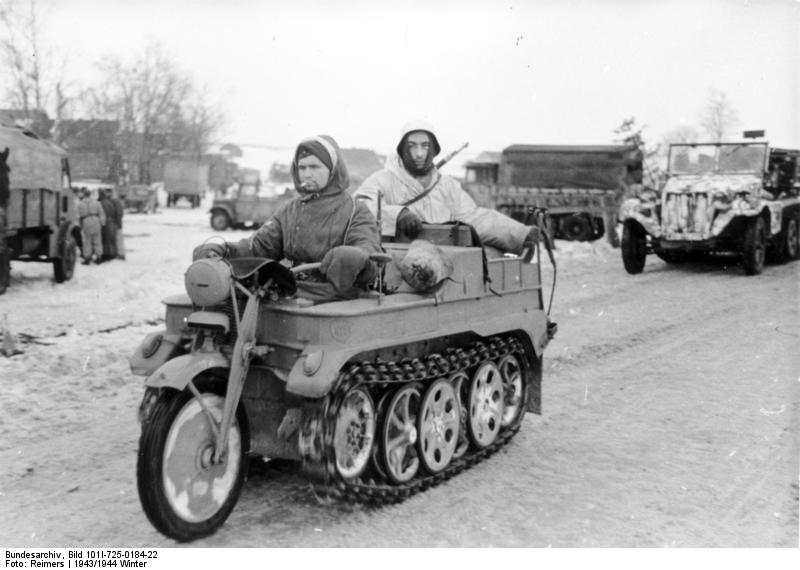
\includegraphics[width=.40\textwidth]{moto_tractora_orig.jpg}
}
\qquad
\subfigure[vehículo militar mixto]{
\label{vmm}
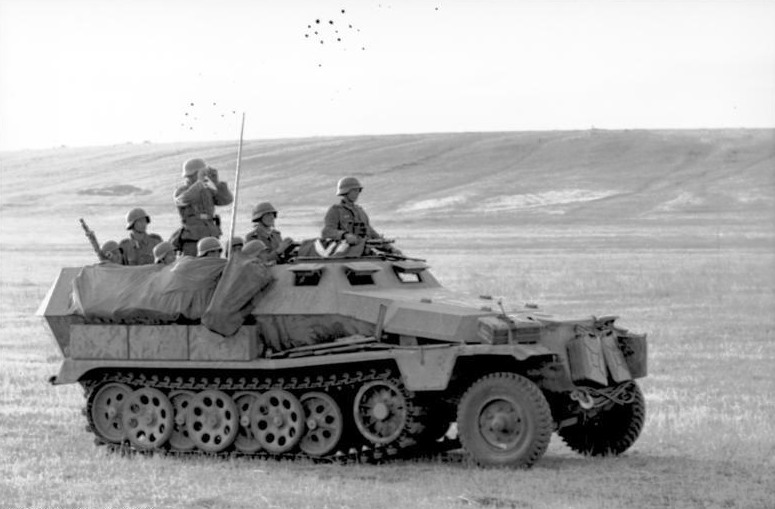
\includegraphics[width=.42\textwidth]{mixto.jpg}
}
}
\caption{\label{fig:militar} La oruga en el uso militar.}
\end{figure}

La {\it mayoría} de las \textit{orugas} forman parte de un
\emph{cinturón} flexible con un conjunto de eslabones rígidos unidos
unos a otros fuertemente. Los eslabones ayudan al vehículo a
distribuir el peso en una superficie mayor que la que hubiera tenido
con el empleo de ruedas, y esto hace que pueda moverse por un número
mayor de superficies sin hundirse debido a su propio peso. Por
ejemplo, la presión que ejerce un automóvil sobre el suelo es igual
aproximadamente a 207 kPa, mientras que las setenta toneladas que pesa
un carro M1 Abrams ejercen una presión sobre el firme de 103 kPa.

\begin{example}
  ~
  \begin{enumerate}
  \item Los tractores con una pala delante son los denominados
    bulldozers, y suelen ser usados en la construcción para remover
    tierra.
  \item Diversos vehículos incorporan la oruga en su mecánica de desplazamiento:
    \begin{enumerate}
    \item Carros de combate.
    \item Ciertos todoterreno de propósito específico, sobre todo de
      uso militar.
    \item Vehículos para el transporte por nieve e hielo.
    \end{enumerate}
  \item El transbordador espacial se transporta a su base de
    lanzamiento mediante una gran oruga transportadora.
  \item El vehículo con oruga más grande del mundo es la rotopala alemana Bagger 288.
  \end{enumerate}
\end{example}